%
% loesung.tex -- Beispiel-File für die Beschreibung der Loesung
%
% (c) 2020 Prof Dr Andreas Müller, Hochschule Rapperswil
%
\section{Lösung
\label{legendre:section:loesung}}
\rhead{Lösung}
\subsection{Anfangswerte
\label{legendre:subsection:anfangswerte}}
Jede Rekursionsbeziehung braucht ihre Anfangswerte.
Sowohl für die $l$-Rekursion \eqref{legendre:recurrence-l} als auch für die $m$-Rekursion \eqref{legendre:recurrence-m} werden je zwei Anfangswerte benötigt.
Für die $l$-Rekursion \eqref{legendre:recurrence-l} werden die Anfangswerte $P^{l}_{l}(x)$ und $P^{l}_{l+1}(x)$ benötigt.
Für die $m$-Rekursion \eqref{legendre:recurrence-m} wird mittels Anfangswert $P^{l}_{l}(x)$ die beiden weiteren Anfangswerte $P^{l}_{l+1}(x)$ und $P^{l+1}_{l+1}(x)$ berechnet.
Diese Anfangswerte lassen sich mittels den Formeln
% Anfangswerte
\begin{equation}
\begin{aligned}
P^{l}_{l}(x)
&=(-1)(2l-1)!!(1-x^2)^{l/2},\\
% Anfangswert P^{l}_{l+1}
P^{l}_{l+1}(x)
&=x(2l+1)P^{l}_{l}(x),\\
% Anfangswert P^{l+1}_{l+1}
P^{l+1}_{l+1}(x)
&=-(2l+1)\sqrt{1-x^2}P^{l}_{l}(x)
\label{legendre:anfangswerte}
\end{aligned}
\end{equation}
berechnen, die sich aus der geschlossenen Form \eqref{legendre:geschlosseneform} herleiten lassen.
Bei der Berechnung des Anfangswertes $P^{l}_{l}(x)$ gilt es zu beachten, dass $!!$ für die Doppelfakultät steht und nicht für die Fakultät der Fakultät.
Im Gegensatz zur einfachen Fakultät werden bei der Doppelfakultät nur die geraden, respektive ungeraden Faktoren zwischen $1$ und der Zahl selber berücksichtigt.
Berechnen lässt sich die Doppelfakultät wie folgt:
\begin{equation}
k!! = 
\begin{cases}
1 \cdot 3 \cdot \ldots \cdot k & \text{falls $k$ ungerade}\\
2 \cdot 4 \cdot \ldots \cdot k & \text{falls $k$ gerade}
\end{cases}
\label{legendre:doppelfakultaet}
\end{equation}

In der Einleitung \ref{legendre:section:einleitung} wurde bereits erwähnt, dass die Rekursionsformeln weniger Rechenaufwand benötigen als die Formel für die geschlossene Form \eqref{legendre:geschlosseneform}.
Dies gilt auch noch unter Einbezug dieser Anfangswerte.

\subsection{$m$-Rekursion
\label{legendre:subsection:mrichtung}}
Für die Abbildung \ref{legendre:fig:plot-m} wurde das zugeordnete Legendrepolynom mit Grad 50 und Ordnung 3 mittels der $m$-Rekursion \eqref{legendre:recurrence-m} berechnet.
Die Anfangswerte $P^{l}_{l+1}(x)$ und $P^{l+1}_{l+1}(x)$ geben vor, dass bei Verwendung dieser Rekursionsbeziehung diese in negativer $m$-Richtung verläuft.
Dazu muss die Formel für die $m$-Rekursion \eqref{legendre:recurrence-m} nach $P^{m-1}_{l}(x)$ umgeformt werden.
Daraus entsteht die neue Formel für die $m$-Rekursion:  
% umgeformte Rekursionsformel in m-Richtung
\begin{equation}
P^{m-1}_{l}(x)
= \left[ \frac{2mxP^{m}_{l}(x)}{- \sqrt{1-x^2}}-P^{m+1}_{l} \right]
\frac{1}{(l+m)(l-m+1)} .
\label{legendre:recurrence-m-neu}
\end{equation}
Wird die umgeformte Rekursionsgleichung \eqref{legendre:recurrence-m-neu} auf numerische Instabilität untersucht, fällt sofort der Term $\sqrt{1-x^2}$ auf.
Dieser Term deutet darauf hin, dass nahe an den Intervallsgrenzen ($x \rightarrow \pm 1$) Auslöschung auftreten kann.
Dies alleine ist noch nicht allzu schlimm.
Jedoch ist es so, dass die zugeordneten Legendrepolynome für $m>0$ an den Intervallsgrenzen Null ergeben.
Das heisst, dass die Differenz in der eckigen Klammer nahe den Intervallsgrenzen in etwa Null ergibt.
Der Term $\sqrt{1-x^2}$, welcher von Auslöschung betroffen ist, wird nahe den Intervallsgrenzen sehr klein und bläst somit den Term $2mxP^{m}_{l}(x)$ auf, welcher dadurch selbst fehlerhaft wird.
Die Differenz in der eckigen Klammer unterliegt somit einer quasi-Auslöschung.
In der eckigen Klammer werden zwei fast gleich grosse Terme voneinander subtrahiert, wobei der erste Term durch die Auslöschung und das Aufblasen durch $\sqrt{1-x^2}$ selbst stark fehleranfällig ist.

Es stellt sich nun die Frage, warum diese numerische Instabilität nicht im Graphen \ref{legendre:fig:plot-m} ersichtlich ist, wie beispielsweise in dem Graphen \ref{legendre:fig:wolframalpha} den Wolfram Alpha erstellt.
Eine Antwort darauf liefert der Term $\frac{1}{(l+m)(l-m+1)}$, welcher einen positiven Einfluss auf numerischer Fehler hat.
Dadurch, dass die Rekursionsgleichung zwei Anfangswerte hat, ist $l\geq m+2$ gegeben.
Damit lässt sich der Nenner dieses Terms auf $\geq 6$ abschätzen, was wiederum bedeutet, dass $\frac{1}{(l+m)(l-m+1)} \leq \frac{1}{6}$ ist.
Dadurch verkleinert sich der Wert der Differenz in der eckigen Klammer der Rekursionsgleichung und ein Teil des Fehlers wird somit eliminiert.
Einige fehlerhafte Stellen hinter dem Komma verschwinden somit.
Diese Rekursionsgleichung bleibt jedoch fehleranfällig nahe den Intervallsgrenzen, falls numerische Fehler aus einer anderen Quelle einfliessen, wie beispielsweise fehlhafte oder ungenaue Anfangswerte.

\subsection{$l$-Rekursion
\label{legendre:subsection:lrichtung}}
Für die Abbildung \ref{legendre:fig:plot-l} wurde ebenfalls das zugeordnete Legendrepolynom mit Grad 50 und Ordnung 3 berechnet, jedoch mittels $l$-Rekursion \eqref{legendre:recurrence-l}.
Die Anfangswerte $P^{l}_{l}(x)$ und $P^{l}_{l+1}(x)$ zeigen, dass die Rekursion in positiver $l$-Richtung verläuft.
Daher muss bei der Gleichung \eqref{legendre:recurrence-l} für die $l$-Rekursion nur noch der Faktor $(l-m+1)$ auf die rechte Seite gebracht werden.
Dies führt zur neuen Formel für die $l$-Rekursion: 
% umgeformte Rekursionsformel in l-Richtung
\begin{equation}
P^{m}_{l+1}(x)
= \frac{(2l+1)xP^{m}_{l}(x)-(l+m)P^{m}_{l-1}(x)}{(l-m+1)} .
\label{legendre:recurrence-l-neu}
\end{equation}
Im Gegensatz zur $m$-Rekursion ist der Term $\sqrt{1-x^2}$ in der Formel für die $l$-Rekursion \eqref{legendre:recurrence-l-neu} nicht vorhanden.
Auch sonst ist kein Term vorhanden, der nahe den Intervallsgrenzen eine numerische Instabilität hervorrufen könnte.
Jedoch gilt es noch die Faktoren vor den zugeordneten Legendrepolynomen zu untersuchen.
Diese beiden Faktoren sind $\frac{(2l+1)}{(l-m+1)}$ und $\frac{(l+1)}{(l-m+1)}$.
Gegeben durch die Anfangswerte ist mit dem gleichen Argument wie im vorherigen Abschnitt \ref{legendre:subsection:mrichtung} wieder gegeben, dass $l\geq m+2$ ist.
Daraus lässt sich ableiten, dass $\frac{(2l+1)}{(l-m+1)}\geq 1$ für $m>0$ ist und dass $\frac{5}{3}\leq \frac{(l+1)}{(l-m+1)}<2$.
Da die beiden Faktoren jeweils $\geq 1$ sind, bedeutet dies, dass die Fehler in den Polynomen $P^{m}_{l}$ und $P^{m}_{l-1}$ vergrössert werden.
Daraus lässt sich schliessen, dass diese Rekursionsbeziehung fehleranfällig ist, falls numerische Fehler aus einer anderen Quelle einfliessen, wie beispielsweise fehlerhafte oder ungenaue Anfangswerte.

\subsection{Welche Rekursionsformel soll nun verwendet werden?
\label{legendre:subsection:welche}}
Es stellt sich die Frage, welche der beiden Rekursionsformeln verwendet werden soll?
Die Formel für die $l$-Rekursion \eqref{legendre:recurrence-l-neu}?
Oder doch die Formel für die $m$-Rekursion \eqref{legendre:recurrence-m-neu}?
Denn obwohl die beiden Graphen, welche mittels $l$-Rekursion (Abbildung \ref{legendre:fig:plot-l}) respektive mittels $m$-Rekursion (Abbildung \ref{legendre:fig:plot-m}) erstellt wurden, optisch gleich aussehen, gibt es Unterschiede.
Diese Unterschiede sind in der Abbildung \ref{legendre:fig:plot-diff} ersichtlich.
Der Graph in dieser Abbildung zeigt die Differenz der berechneten Werte für das zugeordnete Legendrepolynom mit $l=50$ und $m=3$ zwischen der Berechnung mittels $l$-Rekursion und der Berechnung mittels $m$-Rekursion.
Es ist deutlich zu sehen, dass sich die beiden Rekursionsformeln nahe den Intervallsgrenzen unterscheiden.
Die Analyse der $m$-Rekursion aus Abschnitt \ref{legendre:subsection:mrichtung} lässt vermuten, dass diese Rekursionsbeziehung dafür verantwortlich ist.
Dies spricht dafür, die $l$-Rekursion zu verwenden.
Ein weiterer Punkt, der für die $l$-Rekursion spricht, ist, dass die GNU Scientific Library \cite{legendre:gsl} diese Implementation, mit den gleichen Anfangswerten wie in Abschnitt \ref{legendre:subsection:anfangswerte} beschrieben, verwendet.
Die Implementation der GNU Scientific Library wird allgemein als numerisch stabil angesehen.
% Plot in l-Richtung
\begin{figure}[!ht]
\centering
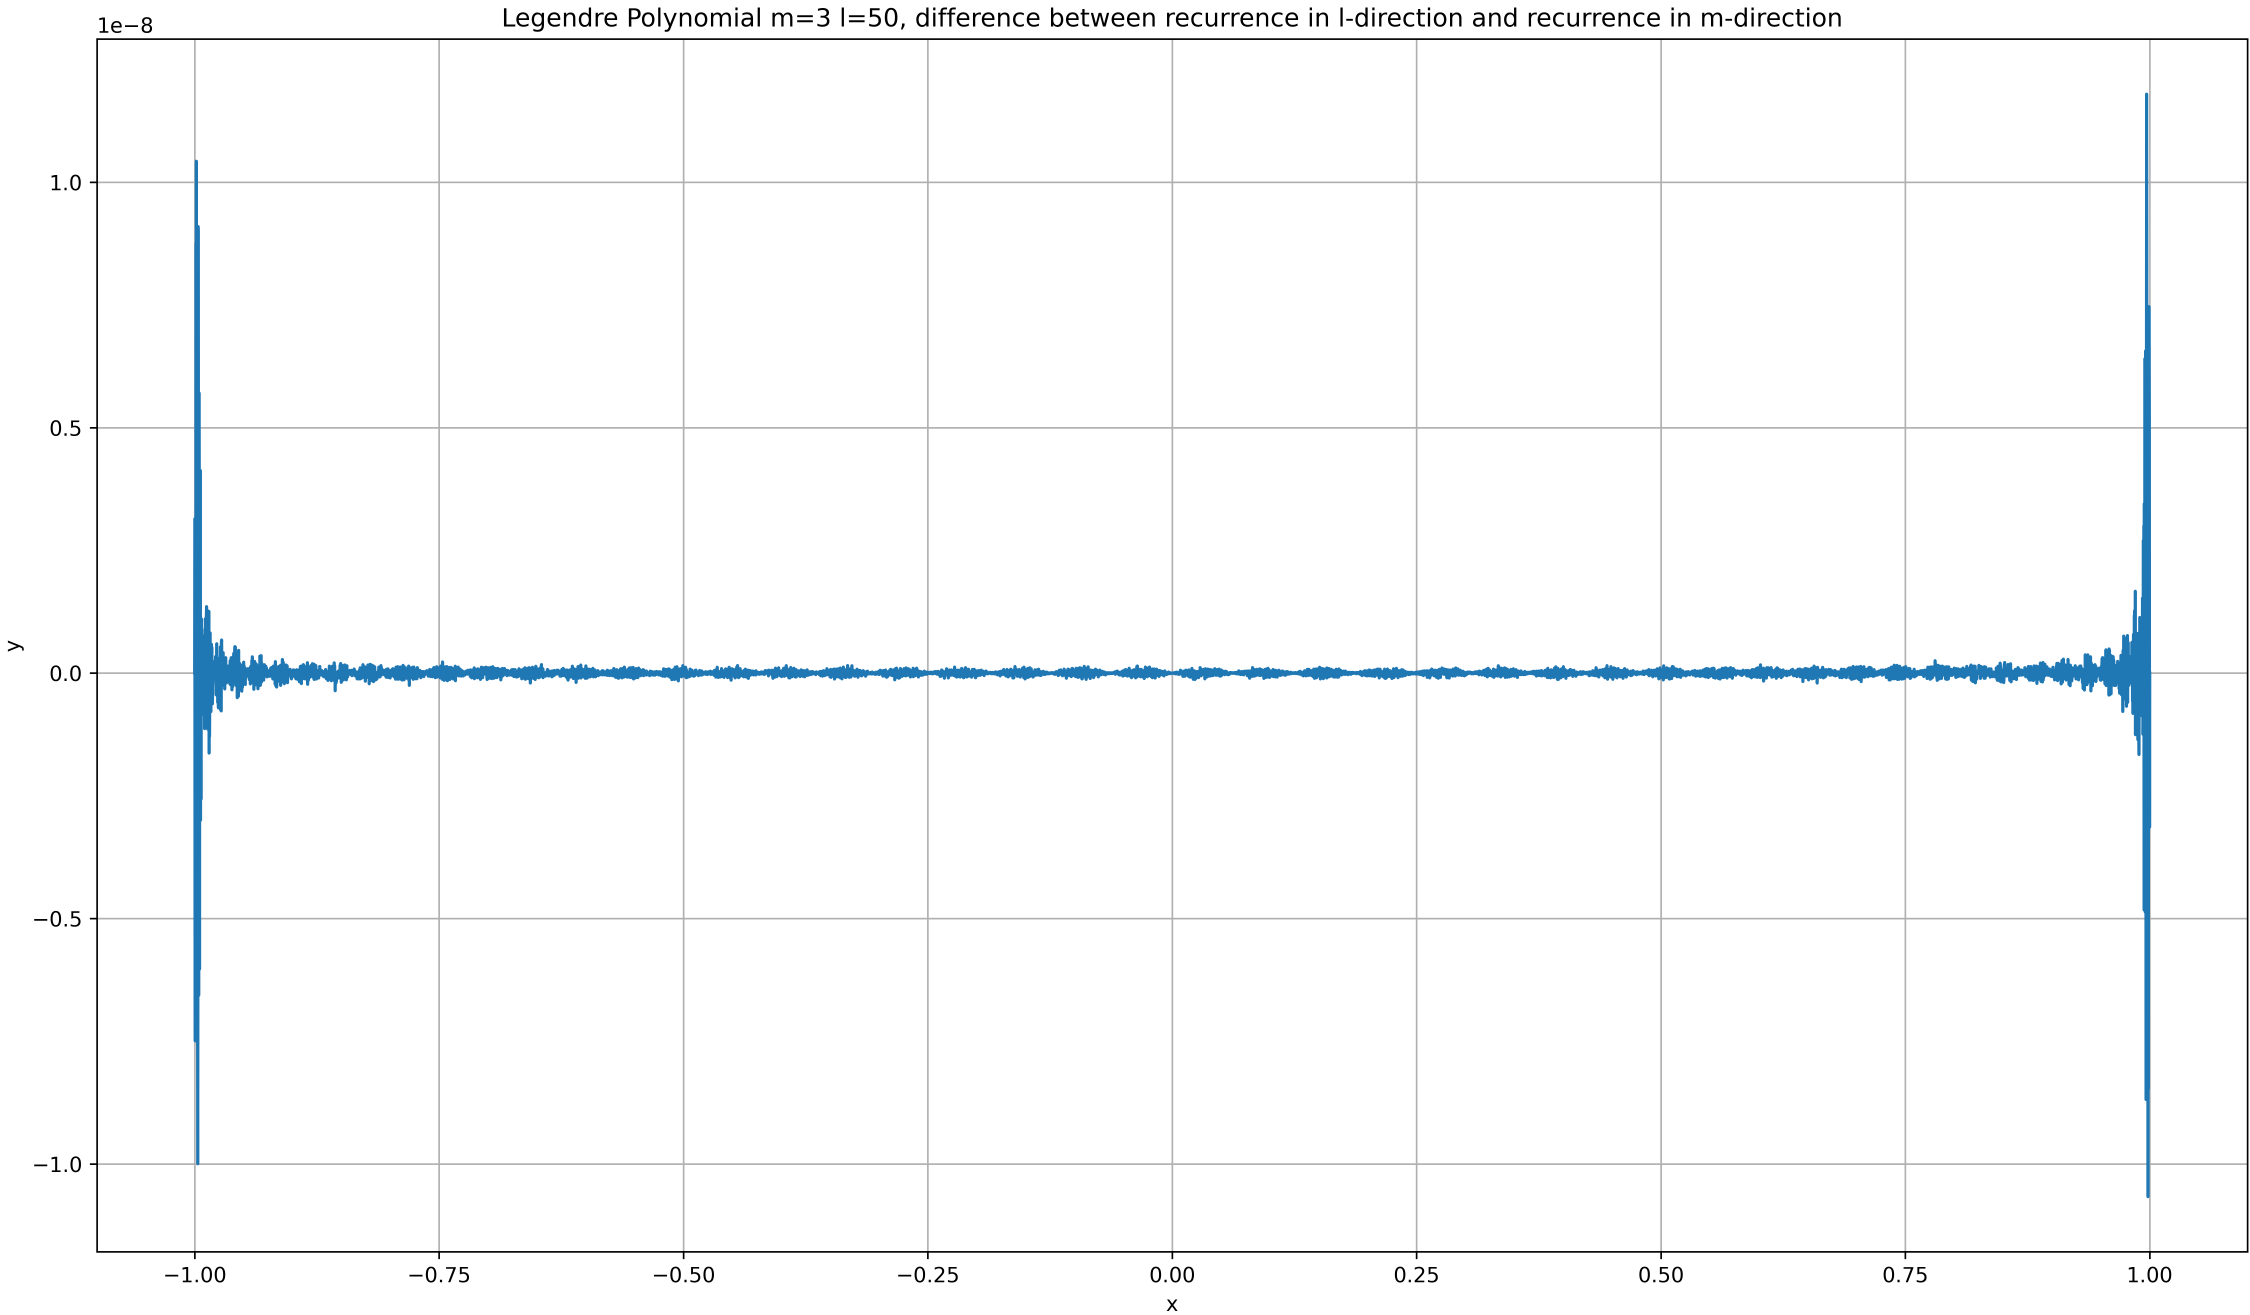
\includegraphics[width=1.0\linewidth]{papers/legendre/plots/plot_diff_l_m_small.png}
\caption{Differenz zweier zugeordneten Legendrepolynome mit \texorpdfstring{$l=50$}{l=50} und \texorpdfstring{$m=3$}{m=3}, einmal berechnet mittels \texorpdfstring{$l$}{l}-Rekursion und einmal berechnet mittels \texorpdfstring{$m$}{m}-Rekursion.}
\label{legendre:fig:plot-diff}
\end{figure}
